\documentclass{beamer}
\usetheme[titlepagelogo=../img/logo-unicam,% Logo for the first page
		  language=english,
		  bullet=triangle,
		  color=green,
          secondsupervisor=true,
          secondlogo=true,
          %assistantsupervisor=true,
         ]{TorinoTh}
         
\usepackage[beamer,customcolors]{hf-tikz}
\hfsetfillcolor{alerted text.fg!10}
\hfsetbordercolor{alerted text.fg}

\author{Piermichele Rosati}
\rel{Dr. Emanuele Laurenzi}
\secondsupervisor{Prof. Michela Quadrini}
%\assistantsupervisor{Dr. James Allan}
\title{\textit{\small HAI-BEMS:\\A Hybrid Artificial Intelligent approach for energy consumption in\\ Building Energy Management Systems}}
\ateneo{\scriptsize University of Camerino \\\&\\ University of Applied Sciences and Arts Northwestern Switzerland}
\date{Ms Thesis - Intermediate Evaluation\\\today}
\titlepagesecondlogo{../img/logo-fhnw}

%%% to remove square brackets from citations %%%
\makeatletter
\def\@biblabel#1{}
\renewcommand\@cite[2]{{#1\if@tempswa,\nolinebreak[3] #2\fi}}
\makeatother
%%%%%%

\begin{document}

\addtobeamertemplate{frametitle}{}{%
\begin{tikzpicture}[remember picture,overlay]
\node[anchor=west,yshift=-20pt] at (current page.north west) {
\includegraphics[height=1.1cm]{../img/logo-unicam-notext.png}};
\node[anchor=north east,yshift=-5pt] at (current page.north east) {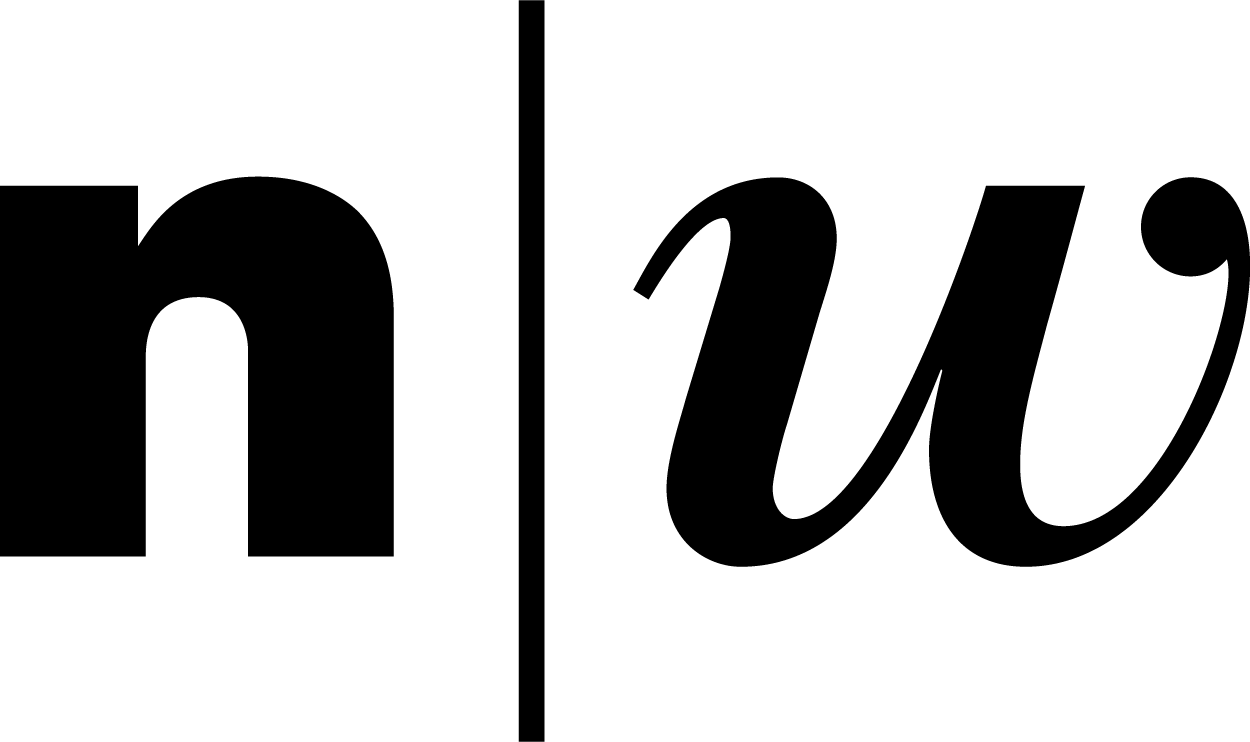
\includegraphics[height=0.9cm]{../img/logo-fhnw-notext.png}};
\end{tikzpicture}
\vspace{-0.5cm}
}

\titlepageframe

\setbeamertemplate{section in toc}[sections numbered]
\setbeamertemplate{subsection in toc}[subsections numbered]
\setbeamercolor{section in toc}{fg=forestgreen}
%\setbeamercolor{subsection in toc}{fg=red}
\setbeamerfont{bibliography item}{size=\footnotesize}
\setbeamerfont{bibliography entry author}{size=\footnotesize}
\setbeamerfont{bibliography entry title}{size=\footnotesize}
\setbeamerfont{bibliography entry location}{size=\footnotesize}
\setbeamerfont{bibliography entry note}{size=\footnotesize}

%%% showing outline before each section %%%
% \AtBeginSection[]
% {
% \begin{frame}<beamer>
% \frametitle{Outline}
% \tableofcontents[currentsection]
% \end{frame}
% }

%%% showing outline only at the beginning %%%
\begin{tframe}{Outline}
    \tableofcontents
\end{tframe}

\section{Introduction}
%\begin{frame}[t,fragile]{In Collaboration with NEST Empa}
    \vspace{-.3cm}
    \begin{figure}[htbp]
        \centering
     
\includegraphics[width=0.5\textwidth]{../img/logo-empa.png}
    \end{figure}
    \begin{itemize}
        \item EMPA (Swiss Federal Laboratories for Material Science and Technology) is a research institute of ETH;
        \vspace{.2cm}
        \item Next Evolution in Sustainable Building Technologies (NEST) is a research focus area of EMPA;
        \vspace{.2cm}
            \begin{itemize}
                \item Objective: Objective: bring new technologies and products on sustainable built environemnt to the market quickly.
                \vspace{.2cm}
                \item Practical R\&D on:
                \begin{itemize}
                    \item Building materials and technologies;
                    \item Thermal insulation;
                    \item Housing facilities;
                    \item \textbf{Energy Management}
                \end{itemize}
            \end{itemize}
    \end{itemize}
\end{frame}
%
\begin{tframe}{Introduction}
%According to~\cite{Manic2016},~
Builing Energy Management Systems (BEMSs) are essential components of modern buildings, tasked with:
    \begin{itemize}
        \item minimizing energy consumption;
        \item maintaining occupants' comfort.
    \end{itemize}
\vspace{0.2cm}
BEMSs control:
\begin{itemize}
    \item Heating, Ventilation, and Air Conditioning (HVAC); %HCVA's primary components (air handling units, chillers, heating elements)
    \item lightning systems.
\end{itemize}
\vspace{0.2cm}
A BEMS implements Internet of Things, Digital Twin and Artificial Intelligence.
\end{tframe}
%
\section{Problem Statement}
\begin{tframe}{Problem Statement}
The problem faced in this thesis is to extract IoT data from sensors and representing it using own ontologies/KGs.
\vspace{.5cm}
\begin{itemize}
    \item The sensory IoT data produced by BEMSs need significant curation before it can be used meaningfully.
    \item Large buildings could have thousands of sensors, which make data transfer and management challenging; %(\cite{Bae2021});
    \item High engineering work requiring multiple domain experts.
\end{itemize}
\end{tframe}
%
\section{Research Question}
\begin{frame}{Research Question}
    \begin{center}
        \textit{How can a Graph Neural Network (GNN) support IoT data classification in KGs about BEMS?}
    \end{center}
    \begin{itemize}
        \item Objective 1: Study of KGs and their applications;
        \item Objective 2: Review of approaches found in the literature, then review of KGs and AI methodologies, in
        particular NNs;
        \item Objective 3: Evaluate possible improvements to the approaches found;
        \item Objective 4: Develop a hybrid approach based on KGs and GNNs.
    \end{itemize}
\end{frame}
%
\section{Working Progress}
\begin{tframe}{Literature of Knowledge Graphs}
    A \gls{kg} refers to a semantic network graph which is consisted of diverse entities, concepts, and relationships in the real world. %(\cite{Hogan2021});
    %It is used to formally describe various things and their associations in the real world.
    \vspace{0.2cm}

    \textbf{Applications}: Social networks, IoT, Healthcare, Search Engines\ldots
    \vspace{0.2cm}

    \begin{minipage}[t]{.5\linewidth}
        \textbf{Benefits of \glspl{kg}:}
        \begin{adv}
            \item Data unification
            \item Easy availability
            \item Semantic meaning
            \item Easier integration
            \item Discovery of hidden patterns
            \item Faster decision making
        \end{adv}
    \end{minipage}%
    \hfill%
    \begin{minipage}[t]{.5\linewidth}
        \textbf{Challenges of \glspl{kg}:}
        \begin{disadv}
            \item Knowledge graph embeddings
            \item Knowledge acquisition
            \item Knowledge completion
            \item Knowledge fusion
            \item Knowledge reasoning
        \end{disadv}
    \end{minipage}
\end{tframe}
%
\begin{tframe}{Literature of Graph Neural Networks}
    GNNs are deep learning based methods that operate on graph domain.
    \vspace{0.2cm}

    \textbf{Applications}: Recommender systems, BioInformatics, Computer Vision\ldots
    \vspace{0.2cm}

    \textbf{Tasks:} Node-Level, Edge-Level, Graph-Level.
    \vspace{0.2cm}

    \begin{minipage}[t]{.5\linewidth}
        \textbf{Benefits of GNNs:}
        \begin{adv}
            \item Modeling relational data;
            \item Generalization to\\ arbitrary graphs;
            \item Capturing complex\\ relationships;
            \item Representation learning.
        \end{adv}
    \end{minipage}%
    \hfill%
    \begin{minipage}[t]{.5\linewidth}
        \textbf{Challenges of GNNs:}
        \begin{disadv}
            \item Scalability;
            \item Data quality and noise;
            \item Model interpretability;
            \item Over-smoothing;
            \item Graph isomorphism problem.
        \end{disadv}
    \end{minipage}
\end{tframe}
%
% \begin{tframe}{Application of KGs}
%     \begin{figure}[htbp]
%         \centering
%      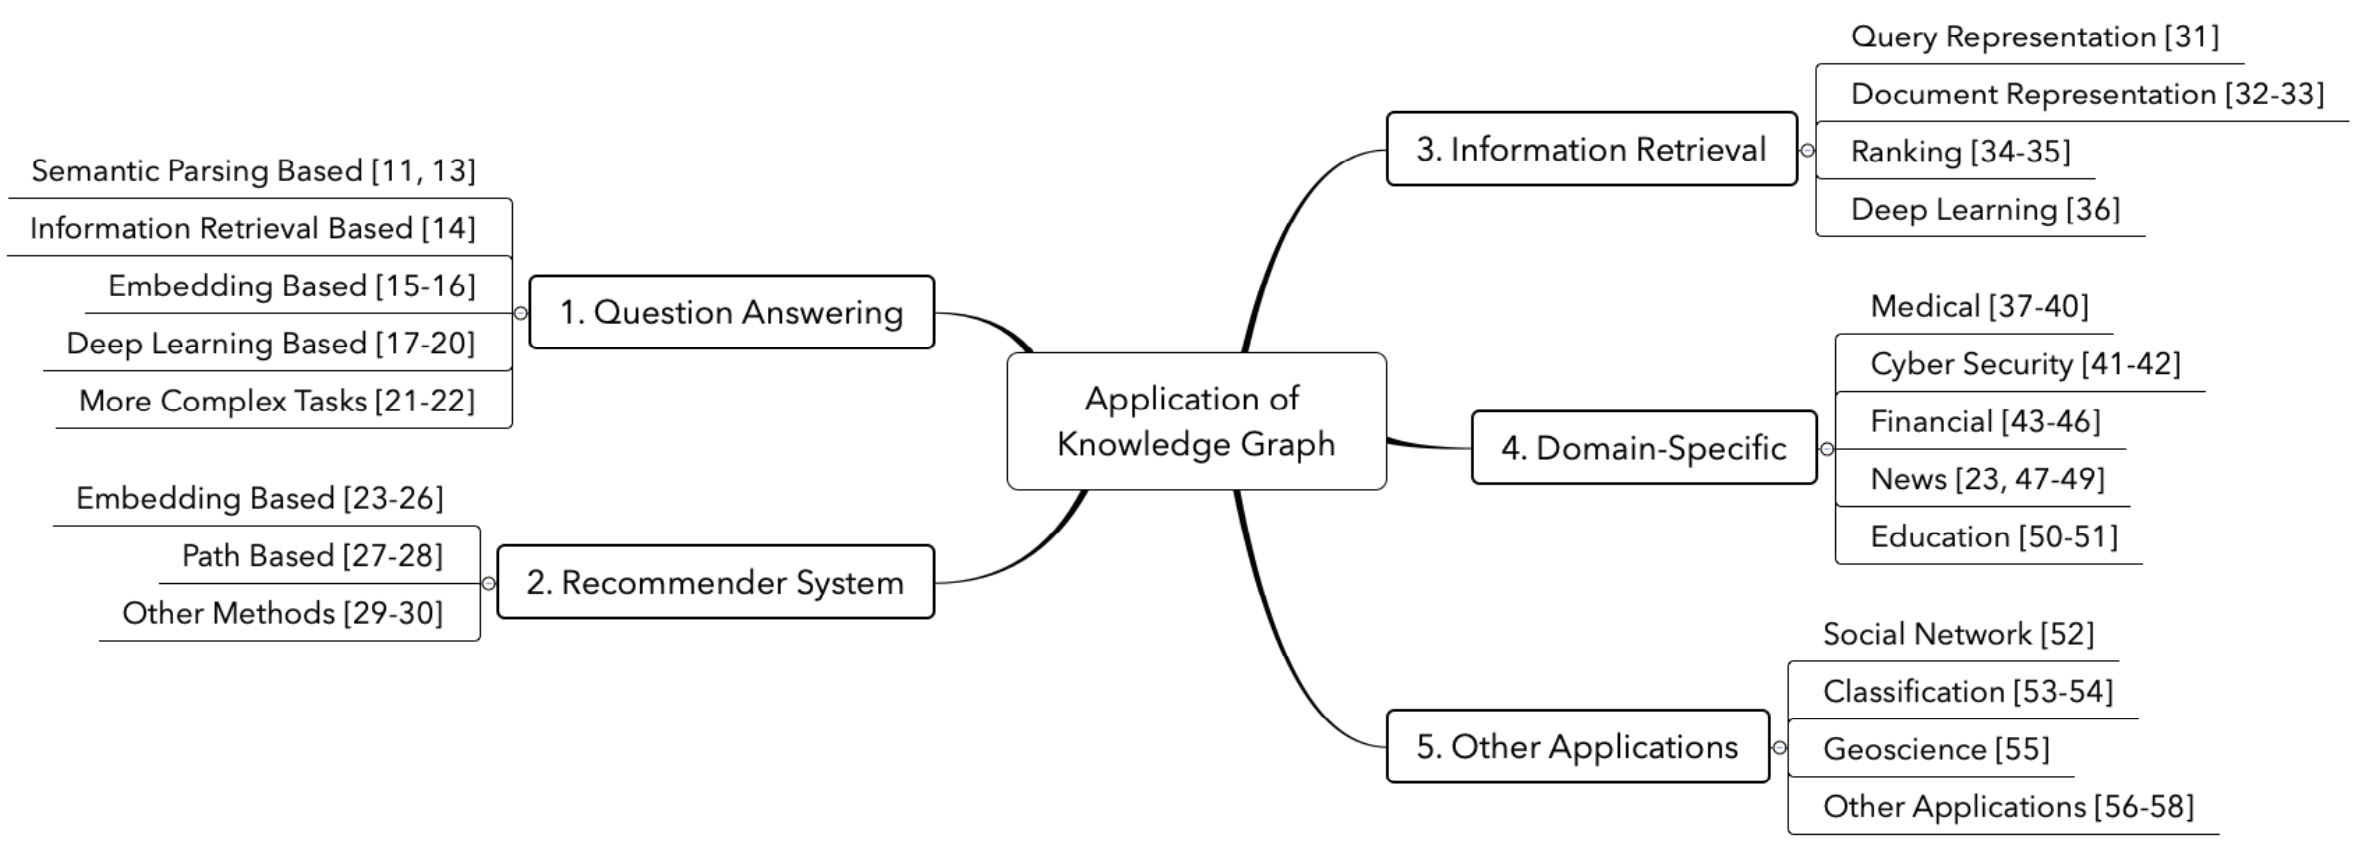
\includegraphics[width=0.9\textwidth]{../img/literature-review/application-field-kg.png}
%      \caption{Application fields of KGs (\cite{Zou2020})}
%     \end{figure}
% \end{tframe}
% \begin{tframe}{Literature of Graph Neural Networks}
% Graph Neural Networks (GNNs) are deep learning based methods that operate on graph domain (non-Euclidean space) (\cite{Wu2021}).
% \newline
% \\ GNNs were introduced when Convolutional Neural Networks (CNNs) failed to achieve optimal results due to the arbitrary size of the graph and complex structure. 
% \newline
% \\ GNN aims to map the node features to node embeddings such that 2 embeddings are ''similar`` if the 2 nodes are ''similar`` in the graph.
% \end{tframe}
% %
% \begin{tframe}{GNN Tasks}
%     \begin{itemize}
%         \item \textbf{Node-Level}: node classification, node regression, node clustering, etc;
%         \item \textbf{Edge-Level}: edge classification and link prediction;
%         \item \textbf{Graph-Level}: graph classification, graph regression, and graph matching.
%     \end{itemize}
% \end{tframe}
% %
% \begin{tframe}{How GNN works}
%     \begin{enumerate}
%         \item \textbf{Message Passing}: is the process of taking node features of the neighbours, transforming them, and ''passing`` them to the source node. This process is repeated, in parallel, for all nodes in the graph. In that way, all neighbourhoods are examined by the end of this step.
%         \item \textbf{Aggregation}: is the process to ''combine`` the transformed messages and the source node together;
%         \item \textbf{Update}: using these aggregated messages, the GNN layer now has to update the source node $\mathnormal{i}$'s features. At the end of this update step, the node should not only know about itself but its neighbours as well. This is ensured by taking the node $\mathnormal{i}$'s feature vector and combining it with the aggregated messages.
%     \end{enumerate}
% \end{tframe}
% %
% \begin{tframe}{The Message Passing Neural Network (MPNN)}
% The MPNN is the most general GNN model:
% \begin{align*}
%     x_i' = \psi(x_i,~\sigma_{j \in N(i)}~ \phi(x_{i},e_{ij},x_j))
% \end{align*}
% where:
% \begin{itemize}
%     \item $\phi$ is a differentiable \textbf{message} funtion;
%     \item $\sigma$ is a permutation-invariant aggregation function (sum, average, etc.)
%     \item $\psi$ is a differentiable \textbf{update} function;
% \end{itemize}
% \end{tframe}
%
\begin{tframe}{Meeting with Domain Experts}
\begin{itemize}
    \item Stakeholders presentation;
    \item BEMS domain details;
    \item Data representation;
    \item Key challenges.
\end{itemize}
\end{tframe}
%
\begin{tframe}{Literature of Knowledge Graph Completion}
\vspace{-.3cm}
Current real-world KGs are usually incomplete and need an inference engine to predict links and complete the missing facts among entities available in the KG.
\newline
\\Knowledge Graph Completion (KGC) is one of the popular technologies for knowledge supplement. 
\vspace{0.1cm}

\begin{itemize}
    \item \textbf{Link Prediction:} aims to predict missing relationships between entities in a graph;
    
    % \begin{minipage}[t]{.5\linewidth}
    %     \textbf{Benefits:}
    %     \begin{adv}
    %         \item Data augmentation;
    %     \end{adv}
    % \end{minipage}%
    % \hfill%
    % \begin{minipage}[t]{.5\linewidth}
    %     \textbf{Challenges:}
    %     \begin{disadv}
    %         \item Scalability, Data sparsity, Bias, ;
    %     \end{disadv}
    % \end{minipage}
    % \vspace{.1cm}
    \item \textbf{Knowledge Graph Embedding (KGE)}: is a representation of a KG element into a continuous vector space;
    % \begin{minipage}[t]{.5\linewidth}
    %     \textbf{Benefits:}
    %     \begin{adv}
    %         \item GNNs models learn\\ powerful embeddings by\\ using topological structures\\ of KGs;
    %     \end{adv}
    % \end{minipage}%
    % \hfill%
    % \begin{minipage}[t]{.5\linewidth}
    %     \textbf{Challenges:}
    %     \begin{disadv}
    %         \item Treat each triple independently;
    %         %\item fail to cover the complex inherently implicit information in the local neighborhood of a triple;
    %         \item Fail to cover the complex inherently implicit information.
    %     \end{disadv}
    % \end{minipage}
    \item \textbf{GNNs} have been recently applied in KGs to learn powerful embeddings by using topological structures in the KGs.
\end{itemize}
\end{tframe}
%
\begin{tframe}{Future Directions}
    \begin{itemize}
        \item Meeting with domain experts for Data collection;
        \item Idea: Ontology schema classes $\rightarrow$ instances;
        \item Apply/Adapt Encoder-Decoder and Attention Mechanisms for KGC:
        \begin{itemize}
            \item R-GCN: locality-sensitive embeddings;
            \item WGCN: breaking into subgraphs;
            \item RGHAT: relational and entity level attention.
        \end{itemize}
        \item Dataset construction;
        \item HAI development:
        \begin{itemize}
            \item Data preparation;
            \item GNN Model selection;
            \item GNN Model training;
            \item GNN Model evaluation and validation;
            \item GNN Model deployment.
        \end{itemize}
    \end{itemize}
\end{tframe}
%
% \section*{References}
% \begin{frame}[allowframebreaks]{References}
%     \nocite{*}
%     \bibliographystyle{apalike}
%     \bibliography{bibliography}
% \end{frame}
%
\section{Conclusion}
\begin{tframe}{Conclusion}
    \textbf{Agentic Graph \gls{rag}} was introduced to deliver contextual and explainable recommendations for research collaborators by combining \textbf{\glspl{kg}} and \textbf{\glspl{llm}}.
    
    \vspace{0.5em}
    \textbf{Evaluation Highlights:}
    \begin{itemize}
      \item High-quality and contextual reasoning, reduced hallucinations
      \item Areas needing improvement: \textit{consistency} and \textit{context retrieval}
    \end{itemize}
    
    %\vspace{0.5em}
    \begin{columns}
      \begin{column}{0.52\textwidth}
        \begin{itemize}
          {\scriptsize
          \item This thesis work has been submitted to the \textbf{Society 5.0 conference}%\footnote{\url{https://www.conference-society5.org}}
          \item A journal version is in preparation for submission to the \textbf{Semantic-Web Journal}%\footnote{\url{https://www.semantic-web-journal.net/blog/special-issue-large-language-models-generative-ai-and-knowledge-graphs}}
          }
        \end{itemize}

        %\vspace{0.2cm}

      \end{column}
      \begin{column}{0.4\textwidth}
        %\vspace{-.5cm}
        \begin{figure}[htbp]
          \centering
          \rotatebox{-5}{\fbox{
\includegraphics[width=.75\textwidth]{../img/conclusion/society-paper.png}}}
      \end{figure}
      \end{column}
  \end{columns}
\end{tframe}
\begin{frame}{The End}
    \vspace{-.15cm}

    \begin{figure}[htbp]
        \centering
        
\includegraphics[width=\textwidth]{../img/thankyou-final.png}
    \end{figure}
    %\centering
    %\huge \textbf{Thank you for your attention!}
\end{frame}


\end{document}